\documentclass[a4paper]{article}

\usepackage[english]{babel}
\usepackage[utf8]{inputenc}
\usepackage{amsmath}
\usepackage{graphicx}
\usepackage[colorinlistoftodos]{todonotes}
\usepackage{amsmath}
\usepackage{array}
\usepackage{multirow}
\usepackage{graphicx}
%\usepackage{subfigure}
\usepackage{subcaption}
\usepackage{tikz}
\usepackage{pgfplots}
\usepackage[colorinlistoftodos]{todonotes}
\usepackage[colorlinks=true, allcolors=blue]{hyperref}
\usepackage{placeins}
\usetikzlibrary{arrows}
\usetikzlibrary{intersections}
\usepgfplotslibrary{fillbetween}
\usepackage{setspace}
\usepackage{epstopdf}

\DeclareGraphicsExtensions{.eps,.pdf,.png,.tikz}
\graphicspath{{figs/}}

\newcolumntype{M}[1]{>{\centering\arraybackslash}m{#1}}
\renewcommand\thefootnote{\textcolor{red}{\arabic{footnote}}}

\title{Backpropagation and Hebbian-LMS}

\author{JKP}

\date{\today}

\begin{document}
\section{Notes on Backpropagation and Hebbian-LMS}
\subsection{Softmax output layer}
For classification problems, it maybe be more appropriate to use the \textit{softmax} function rather than the one-out-of-many code in the output layer. With \textit{softmax}, the $i$th neuron in the output layer outputs $y_i = p(x \in K_i)$ i.e., the probability that the the input $x$ is in the $i$th cluster. Training is done to make $p(x \in K_i) = 1$ when $x \in K_i$. Hence, each output neuron is ``responsible'' for a cluster, and it'll give the probability that the input belongs to that cluster. Decisions are made by trusting the neuron that outputs the highest probability. 

The error equation for the softmax layer is given by
\begin{equation}
\epsilon_k = D - \frac{\exp{S}}{\sum\exp{S}}
\end{equation}
where $D$ is the desired response vector and $D_i = 1$ when the input vector belongs to the $i$cluster, otherwise $D_i = 0$. $S$ is the output of the linear combiner. The value $p = \frac{\exp{S}}{\sum\exp{S}}$ is interpreted as a probability vector such that $p_i$ corresponds to the probability that the input vector belongs to the $i$ cluster. Moreover, note that in calculating the error for a single neuron, all neurons in the output layer are used. In the one-out-of-many code, the error calculation for a single neuron doesn't depend on the output of other neurons in the output layer.

Figure~\ref{fig:comp} compares the performance of the softmax output layer with that of the one-out-of-many code. The simulation parameters are detailed in the figure caption. The simulation parameters were not extensively optimized for either case. These results are to be taken simply as examples and not proof of superiority of one method over the other.

\FloatBarrier
\begin{figure}[h!]
	\centering
	\begin{subfigure}[h!]{0.8\textwidth}
		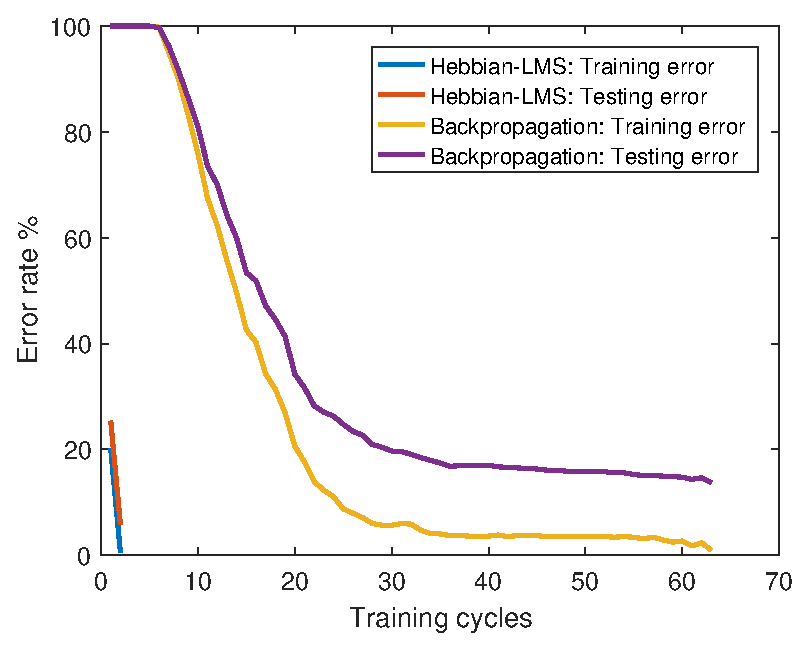
\includegraphics[width=\textwidth]{learning_curve_oom_code.eps}
		\caption{One-out-of-many code output layer. Hebbian-LMS took only 2 training cycles (1.57 sec). Backpropagation took 63 training cycles (33.77 sec).}
		\label{fig:learning_curve_oom_code}
	\end{subfigure}%

	\begin{subfigure}[h!]{0.8\textwidth}
		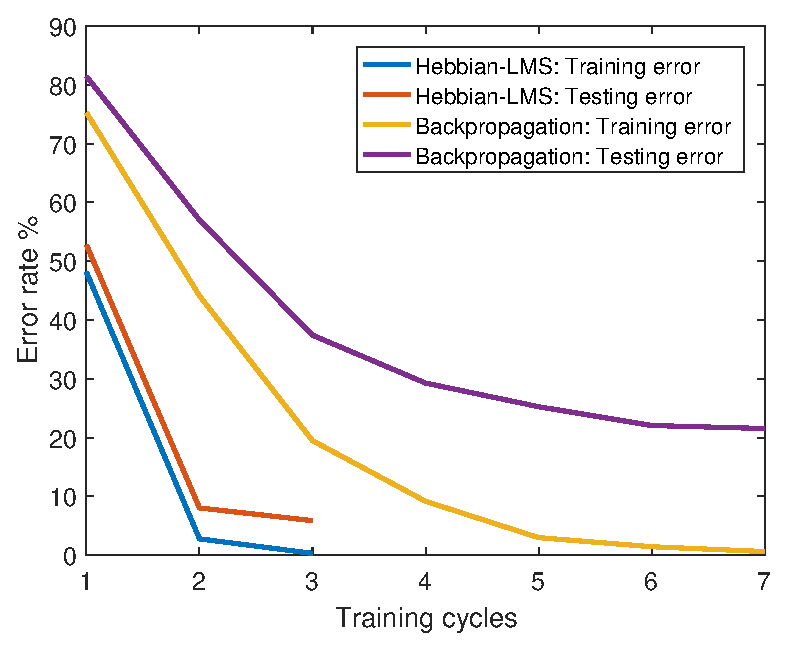
\includegraphics[width=\textwidth]{learning_curve_softmax.eps}
		\caption{Softmax output layer. Hebbian-LMS took 3 training cycles (2.88 sec). Backpropagation took 7 training cycles (3.73 sec).}
		\label{fig:q81a_vel}
	\end{subfigure}
	\caption{Comparison of backpropagation and Hebbian-LMS using (a) one-out-of-many code and (b) softmax output layer. Both networks had 3 hidden layers and 50 neurons per hidden layer. The input vector space had 50 dimensions, 50 clusters, but only 47 clusters were presented during training. 20 patterns from each cluster were used during training, and another 20 patterns during testing. $\rho = 0.2$, where $\rho$ is defined as in the paper. Training was stopped when training error was below $1\%$. }\label{fig:comp}
\end{figure}
\FloatBarrier
	
\subsection{Complexity comparison between Backpropagation and Hebbian-LMS}

This subsection shows how to calculate the number of floating-point operations required by Hebbian-LMS and backpropagation learning algorithms.
	
\subsection{Weights update with backpropagation algorithm}

The backpropagation weights update for the hidden layers can be summarized in the following equations:

\begin{align} \label{eq:bp-eqs1}
\delta^{(l-1)} &= (W^{(l)T}\delta^{(l)})\odot \sigma^\prime (S^{(l-1)}) \\ \label{eq:bp-eqs2}
W^{(l)} &= W^{(l)} + 2\mu\delta^{(l)}Y^{(l-1)} \\ \label{eq:bp-eqs3}
b^{(l)} &= b^{(l)} +  2\mu\delta^{(l)},
\end{align}
where $\odot$ denotes element-wise product of two vectors, and $\sigma^\prime(x)$ is the first derivative of the sigmoid function.
\begin{itemize}
	\item $W^{(l)}$ is a $N_w \times N_w$ matrix of the weights of the $l$th layer. $W_{ij}^{(l)}$ is the $j$th weight of the $i$th neuron.
	\item $b^{(l)}$ is a $N_w \times 1$ vector of the bias weights of the $l$th layer. $b_i^{(l)}$ is the bias weight of the $i$th neuron.
	\item $S^{(l)} = W^{(l)}Y^{(l-1)} + b^{(l)}$ is a $N_w \times 1$ vector corresponding to the output of the adders in the $l$th layer. $S_i^{(l)}$ is the output of the $i$th neuron of the $l$ layer.
	\item $Y^{(l)} = \sigma(S^{(l)})$ is a $N_w \times 1$ vector corresponding to the output of the neurons in the $l$th layer. $Y_i^{(l)}$ is the output of the $i$th neuron of the $l$ layer.
\end{itemize}

By inspecting \eqref{eq:bp-eqs1}--\eqref{eq:bp-eqs3}, we can conclude that the backpropagation algorithm requires the following number of floating-point operations
\begin{align} \nonumber
N_{BP, FB} &= 2(N_w - 1)N_w + N_w~\text{($\delta$ calculation)} \\ \nonumber
& + 3N_w^2~\text{(weights updates)}\\  \nonumber
& + 2N_w~\text{(bias updates)} \\
& = 5N_w^2 + N_w~\text{flops/hidden layer}
\end{align}
This only includes the hidden layers and assumes that the first layer has the same number of inputs as of all other hidden layers. Additional $N_w$ $\sigma^\prime(x)$ operations are required. 

The values of $S^{(l)}$ and $Y^{(l)}$ are calculated in the forward pass, and are assumed to be available during the backward pass. The forward pass performs $S^{(l)} = W^{(l)}Y^{(l-1)} + b^{(l)}$ and $Y^{(l)} = \sigma(S^{(l)})$. Hence, the number of operations in the forward pass is given by
\begin{align}
N_{BP, FF} = 2(N_w-1)N_w + N_w = 2N_w^2 - N_w ~\text{flops/hidden layer}
\end{align}
Additional $N_w$ $\sigma(x)$ operations are required. 

\subsection{Weights update with Hebbian-LMS algorithm}

For Hebbian-LMS, the number of operations required in the forward pass is the same as for backpropagation. For the weights updates, we have 
\begin{align} \label{eq:hlms-eqs1}
\delta^{(l)} &= (Y^{(l)} - \gamma S^{(l)}) \\ \label{eq:hlms-eqs2}
W^{(l)} &= W^{(l)} + 2\mu\delta^{(l)}Y^{(l-1)} \\ \label{eq:hlms-eqs3}
b^{(l)} &= b^{(l)} +  2\mu\delta^{(l)}
\end{align}
For the modified Hebbian-LMS, the first equation is $\delta^{(l)} = -(Y^{(l)} - \gamma S^{(l)})\odot (\sigma^\prime(S^{(l)}) - \gamma)$.

By inspecting \eqref{eq:hlms-eqs1}--\eqref{eq:hlms-eqs3}, we can conclude that the number of floating-point operations is
\begin{align} \nonumber
N_{HLMS} &= 2N_w ~\text{($\delta$ calculation)} \\ \nonumber
& + 3N_w^2~\text{(weights updates)}\\  \nonumber
& + 2N_w~\text{(bias updates)} \\
& = 3N_w^2 + 4N_w~\text{flops/hidden layer}
\end{align}

Table~\ref{tab:num-op} compares the number of floating-point operations required per training cycle for both backpropagation and Hebbian-LMS algorithms. The table shows how many floating-point operations are required in the calculating the outputs of the network (outputs update), and in updating the weights. For large $N_w$ or $N_{hl}$, Hebbian-LMS uses $5/7$ of the number of operations of backprorogation.

\FloatBarrier
\begin{table} [h!]
	\caption{Number of floating-point operations required by the backpropagation and Hebbian-LMS learning algorithms. Additional $N_{hl}N_w~\sigma(x)$ operations are required in the outputs update for both Hebbian-LMS and Backpropagation. Backpropagation also requires additional $N_{hl}N_w~\sigma^\prime(x)$ operations for weight updates. For Hebbian-LMS the weights update operations can be parallelized so that the weights are updated simultaneously for each layer.} \label{tab:num-op}
	\centering
	\begin{tabular}{M{3.5cm}|M{3.5cm}|M{3.5cm}}
		\hline
		Algorithm & Outputs update & Weights update \\
		\hline
		Hebbian-LMS &  $N_{hl}(2N_w^2 - N_w)$ & $N_{hl}(3N_w^2 + 4N_w)$  \\
		Backpropagation & $N_{hl}(2N_w^2 - N_w)$ & $N_{hl}(5N_w^2 + N_w)$ \\
		\hline
	\end{tabular}
\end{table}
\FloatBarrier

\subsection{Parallelization}
In a backpropagation network, training has to be realized in two passes. The forward pass, whereby the outputs of each layer are computed, and the backward pass, whereby the weights of each neuron are updated. Both of these passes have to be realized in a sequential fashion i.e., one layer at a time. In the Hebbian-LMS network, the forward pass still has to be realized sequentially, but the weights of each neuron can be updated independently. Hence, parallelization can be used to achieve extra gains in computational efficiency. This advantage is particularly relevant in today's multi-core computer architectures. 

\end{document}